\documentclass[a4paper, 11pt, twocolumn]{article}
\usepackage[left=1.5cm, top=2.5cm, total={18cm, 25cm}]{geometry}
\usepackage[utf8]{inputenc}
\usepackage[english]{babel}
\usepackage[T1]{fontenc}
\usepackage{graphicx}
\usepackage[nottoc]{tocbibind}
\usepackage[spaces]{url}
\def\UrlBreaks{\do\/\do-}
\usepackage{breakurl}
\usepackage[breaklinks, unicode, hidelinks]{hyperref}
\usepackage[square,numbers]{natbib}

\begin{document}
    \title{\LARGE{Microprocessors and Embedded Systems}\\\huge{Musical instrument simulator}}
        \author{Jakub Bartko \\ \texttt{xbartk07@stud.fit.vutbr.cz} \\ \the\year}
        \date{}
        \maketitle

\section{Introduction}
    The purpose of this project is to design, implement and present a~musical instrument simulator using WeMos D1 R32 UNO ESP32 board.
    
    The implemented functionality includes virtual piano keyboard, song recording and replaying of recorded or prerecorded songs. Whole application, including playing, song manipulation and mode switching is operated with included 3 by 4 keypad. The sound output is handled by connected external speaker.
    
\section{Modes and Controls}
    The listed functionality is devided into 3 main modes: free play, song recording and song playing.
    
    The \texttt{Free Play} mode is implemented to imitate the functionality and operation of a~chromatic harmonica\footnote{\url{https://en.wikipedia.org/wiki/Chromatic\_harmonica}}. It usually consists of several  octaves~--~an octet of notes, usually in C~major, with a side button for playing each note a~semitone higher. The octave (+1~additional note) can be played using keys 1~through~9. The default position is for key 1 to represent middle C. Use keys \#~and *~to shift the octave one note up or down, respectivelly. The "single semitone upshift" can be executed by pressing down the '0' key and desired note key. This way, the possibility of playing any piano note in 3~octaves (21~keys!) is achieved, using only 9~tone and 3~control keys. Press 0 key twice to switch to song mode.
    
    The \texttt{Song Mode} consists of playing prerecorded songs, recording your own using the functionality of Free Play mode and replaying your recordings.
    Insert the desired song code using keys 1~through 9. Press \# key to play the song with specified code.
    
    Switch to \textit{Record Mode} by pressing the *~key while idle in Song Mode. The functionality is equal to the Free Play mode. Stop the recording by pressing the 0~key twice. Enter the 4-digit song code you wish to save it under and press the * key to save the song; or press the \# key to discard the recording. Either of these return you to the Song Menu, from where you can now play your recording under the specified code. A~showcase song~--~simplified Take Me Home, Country Roads by John Denver and et al., recorded by the author of this project, is available under the song code 9999.

        
\section{Implementation}
    The aforementioned functionality is implemented in the \texttt{main.c} file. It makes use of standard \texttt{Arduino} library and the Keypad library\footnote{\url{https://www.arduinolibraries.info/libraries/keypad}} by Mark Stanley and Alexander Brevig.
    
    The main functionality is implemented in the \texttt{loop} function, in which, according to current mode and pressed buttons, the next state is determined. The respective handling of button pressed and switching of modes is implemented in functions with \texttt{handle\_} prefix. The buzzer is manipulated using \texttt{ledcWriteTone} which implements the pulse-width modulation functionality. Tone is set to be played according the \texttt{tone\_list} and pressed/recorded key. After the key release/pause in melody, tone with frequency 0 is set to be played.
        
\section{Demonstration}
    The video demonstration of the project's functionality is available from \href{https://github.com/bix-1/IMP}{\textit{my public repository}}, or directly \href{https://user-images.githubusercontent.com/61697719/146260228-3d847d57-f754-4025-8446-bd0458d8adeb.mp4}{\textit{here}}.
        
\section{Summany and conclusion}
    The goal of this project was to design and implement musical instrument simulator on an ESP32 board. As presented in this document and the attached demonstration, the goals set withing this project have been successfully achieved with no known limitations. Some additional attention has also been given to the user experience, namely by implementing the pseudo multi-touch functionality (no need to lift a~key to press another), user-friendly recording with no need for key-duration input for each individual note, and the ability to store over 7,000 songs.
        
\clearpage
\appendix
\section{Schema}
    \begin{figure}[ht]
    		\centering
    		\includegraphics[width=1 \linewidth]{schema.pdf}
    		\caption{Schema}
    \end{figure}
\vfill\eject
\section{Setup}
    \begin{figure}[ht]
    		\centering
    		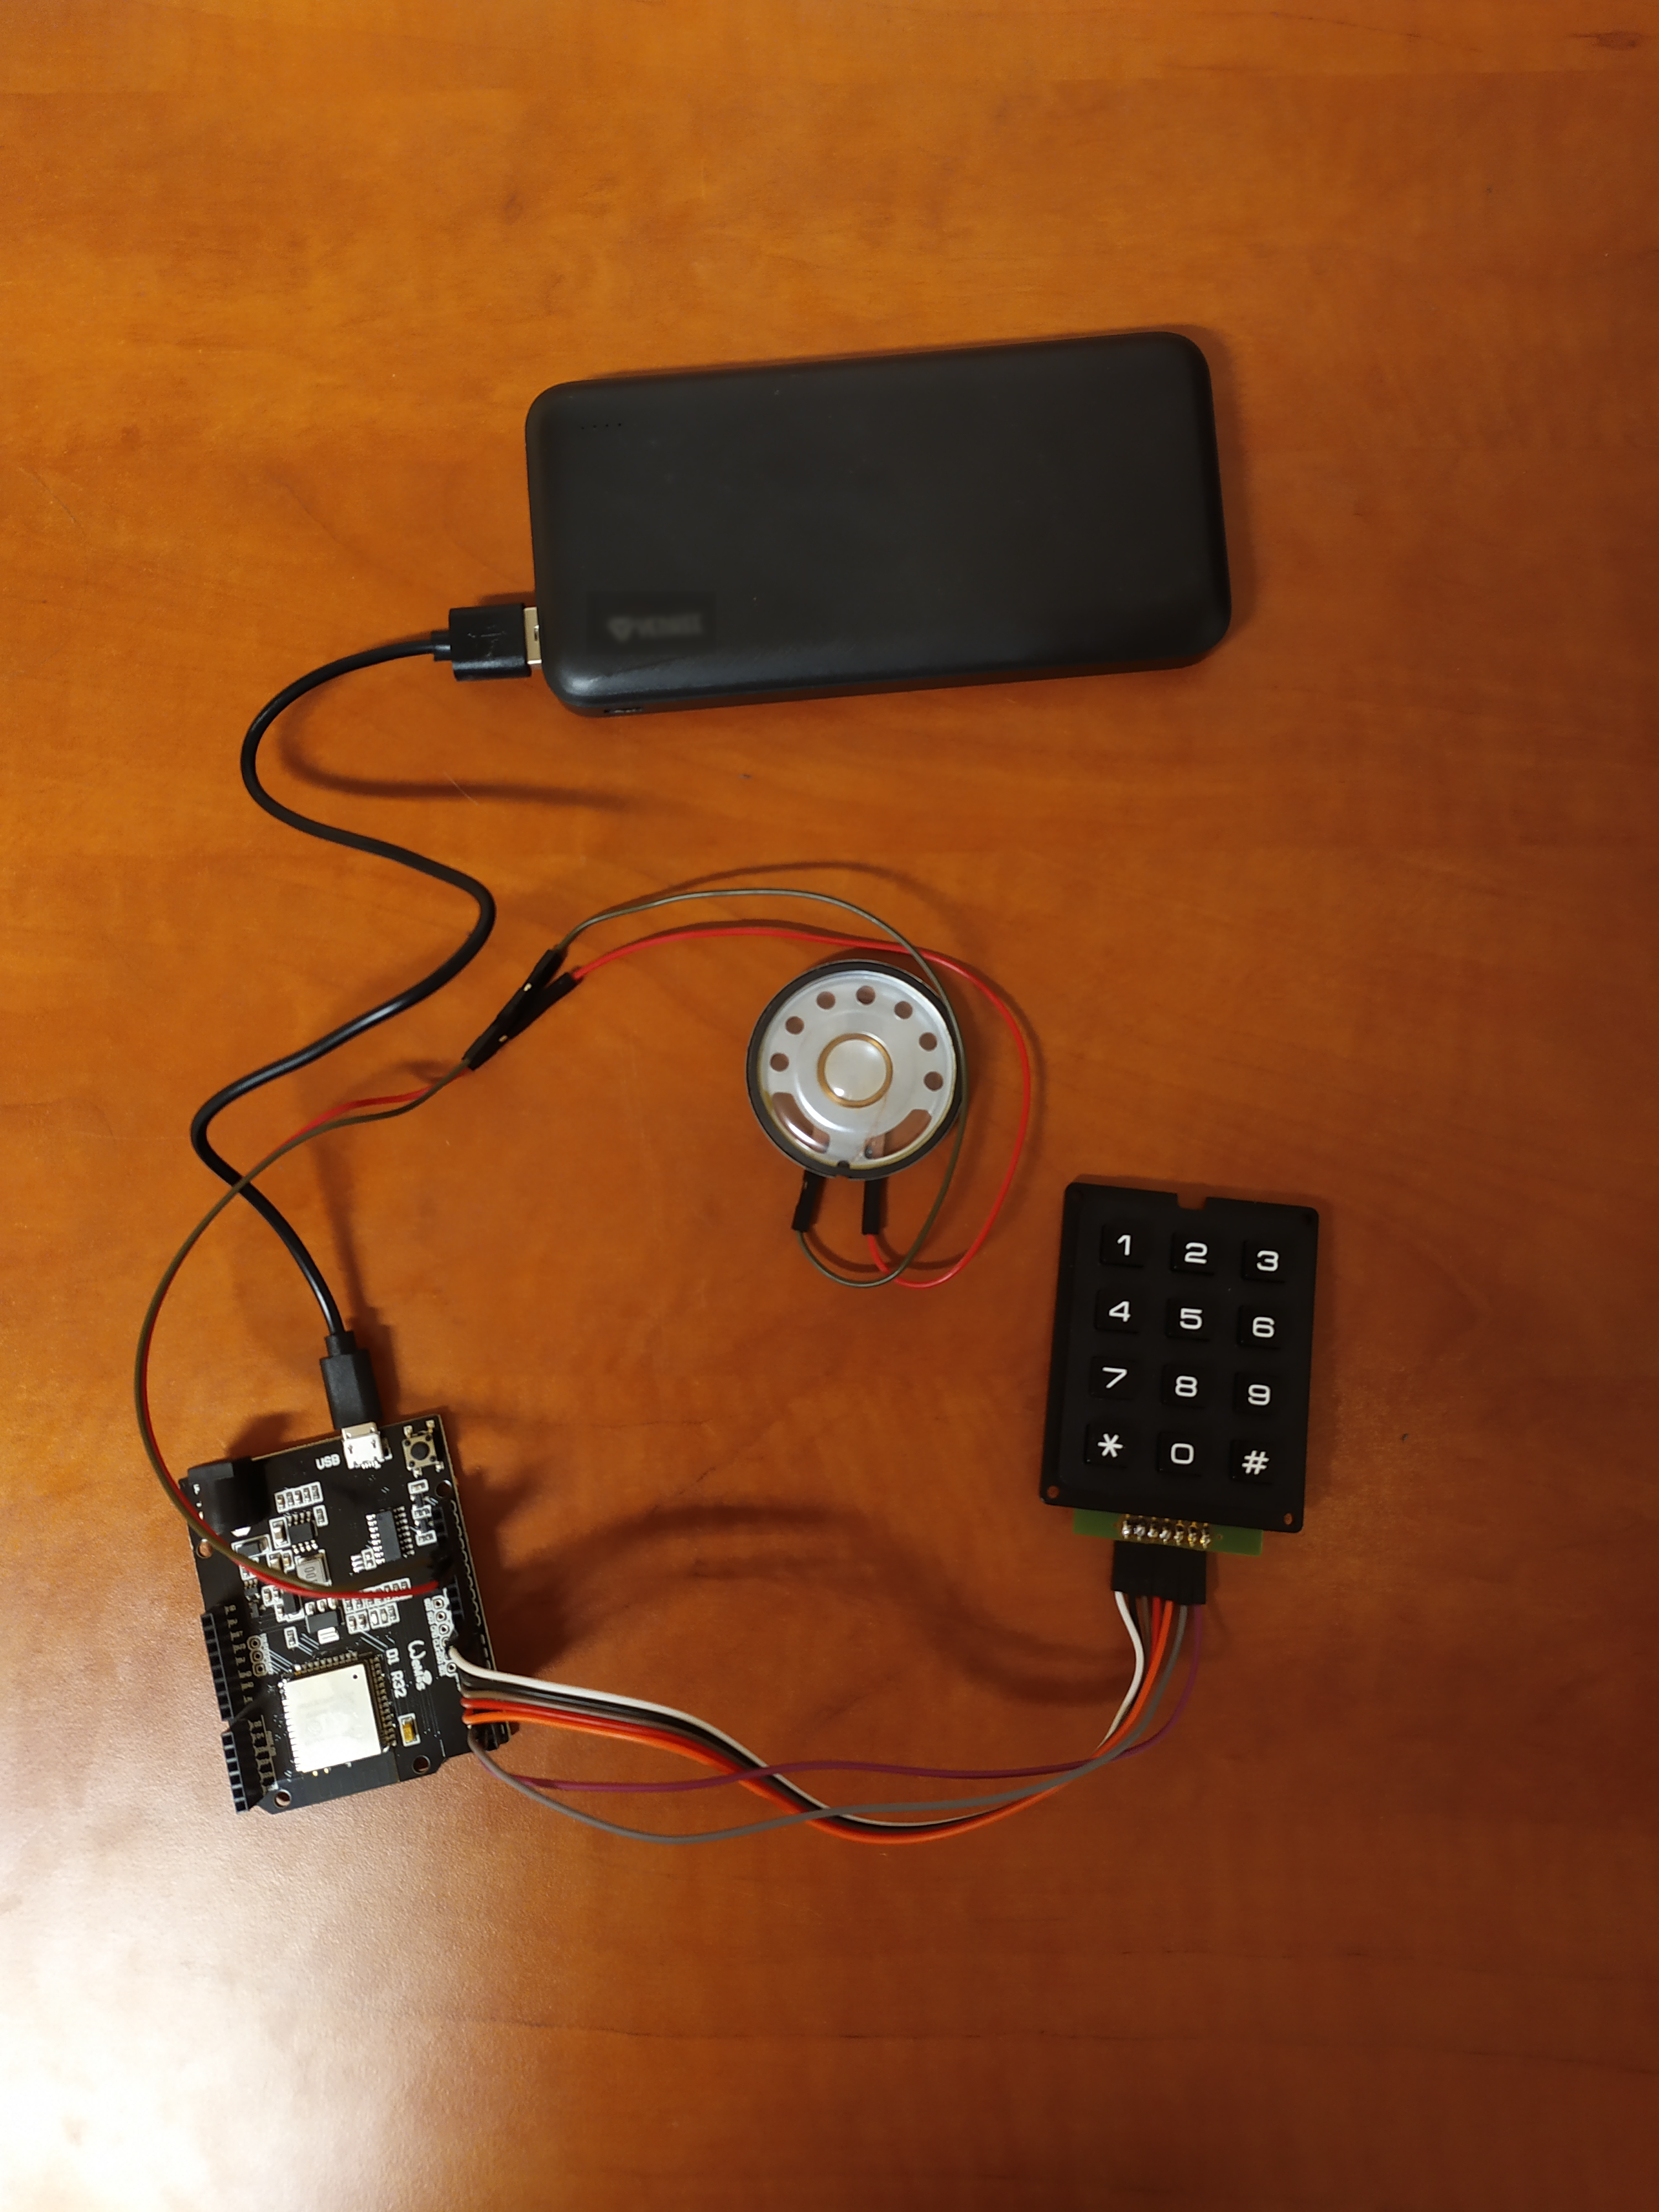
\includegraphics[width=0.8 \linewidth]{setup.png}
    		\caption{Setup}
    \end{figure}
\end{document}
